	\chapter{Inleiding}
	%[comments]
	%Leg in de inleiding van breed naar smal het probleem in zijn context uit.\\
	%Je eindigt de inleiding precies daar waar je het probleem globaal beschreven hebt.\\
	
	Het doel waar naar toe wordt gewerkt in dit onderzoek is om via het S88 timing protocol te communiceren met het RM-88-N schuifregister doormiddel van een NI-FPGA bord te programmeren in de hardware beschrijvingstaal VHDL.
	
	Dit houd in: \\
	- Werkende VHDL code schrijven om de verbinding te leggen met het schuifregister en de betreffende respons op te vangen en weer te geven, zodat er een duidelijk beeld is dat de communicatie tot stand is gebracht. \\
	- Het S88 timing protocol onderzoeken en waarom dit toepasselijk is voor dit onderzoek.
	
	Hier een schematisch beeld van zowel het NI-FPGA bord, als het RM-88-N schuifregister.
	\begin{figure}[h]
		\begin{center}
			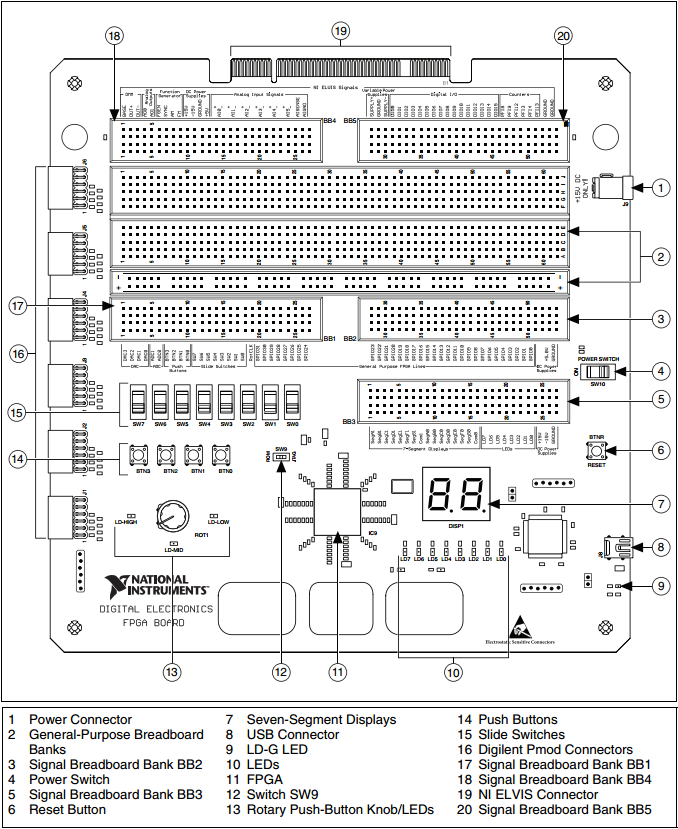
\includegraphics[width=105px]{./img/FPGA.png}\hspace{20mm}
			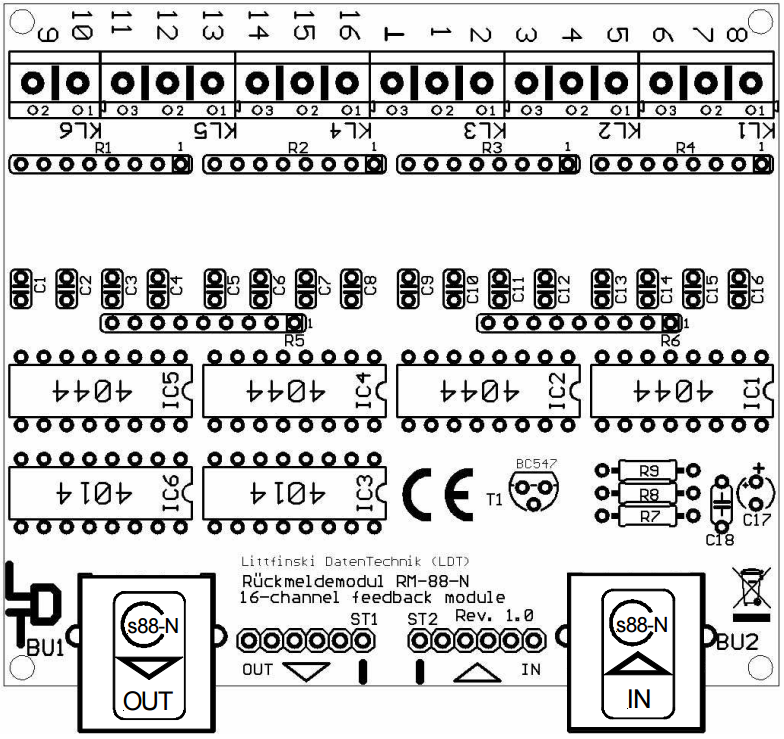
\includegraphics[width=105px]{./img/RM88.png}
			\caption{Schematische weergaven hardware}
		\end{center}
	\end{figure}
	%Dan in het hoofdstuk specificatie geef je alle onderdelen weer die door fabrikanten aangeleverd worden, voor zover van toepassing. (Let op! Dit is een keuze, vaak is er een wisselwerkng tussen je specificatie en je requirements en daarmee de volgorde van de hoofdstukken.)\\
	
	
	
	%Nu komt de probleem stelling met eventuele onderzoeksvragen aan de orde met daarbij de requirements, etc. Een indeling kun je ook op BB vinden. Die is echter niet zaligmakend,\\ aangezien het kan zijn dat het probleem op zich leidt tot onderzoeksvragen die aanleiding geven tot een hardware keuze.\\
	
	
	
	%Uiteindelijk moet in je verslag een hoofdstuk het logische vervolg zijn op het vorige hoofdstuk.\\
	
	

	%Geef ter illustratie in dit hoofdstuk ook schematische weergaves van de hardware (het NI-FPGA bord en het RM88-N bord).\\
	%Hiernaar kun je dan in je tekst verwijzen.